\section{\label{III-B-3}Perspectives d'utilisation}
\titreEntete{Perspectives d'utilisation}

%intro
\begin{citationLongue}
	[L]e rôle central du référentiel va se poursuivre au-delà de [la] réflexion sur l’interopérabilité. En effet, ils sont la pierre angulaire des nouveaux bouleversements autour du \textit{machine learning} et du \textit{deep learning}.\footcite{poupeau_reflexions_2018}
\end{citationLongue}

L'interopérabilité des données --- comprises au sens large, avec les métadonnées et les référentiels --- est une avancée majeure dans la conception des modèles de données. En effet, en plus de résoudre les nombreuses difficultés qui résultaient de la multiplicité des bases de données à l'\ac{ina} et de leur conception par les besoins et les usages qui en étaient faits, la centralisation de ces données et leur interopérabilité ouvre des possibilités quant aux nouveaux usages qu'il est possible d'envisager ou de satisfaire.\\

L'intégration de l'\ac{ina} dans le \textit{big data} est l'une de ces possibilités: l'utilisation de l'intelligence artificielle permet à la fois une amélioration des descriptions déjà réalisées au catalogage, et ainsi que la création de nouvelles descriptions. Plus encore que ces actions sur les métadonnées et la création de descriptions de contenus, l'amélioration de la valorisation des documents de l'\ac{ina} est possible avec le \ldd et l'uniformisation du modèle de données.

\subsection{\label{III-B-3-a}Permettre l’intégration des données issues de la description et de la segmentation de vidéos dans le \ldd : réutilisation des concepts et enrichissement des métadonnées}
\titreEntete{La description automatique de vidéos}
	
La reconnaissance d'entités nommées est un enjeu essentiel dans la description de documents. Cette dernière est facilitée, depuis quelques années, par des outils nés de programme de recherche sur l'extraction d'entités nommées dans les textes. La classification d'images est également une pratique facilitée par des algorithmes développés par des entreprises comme Google ou Amazon. Cependant, l'extraction d'entités nommées dans des vidéos reste peu pratiquée. \index[ref]{led@Linked Enterprise Data (LED)!ldd@Lac de données (INA)}\index[ref]{modelisation@Modélisation!ldd@Lac de données (INA)}L'\ac{ina} ne dispose alors pas d'outils suffisants et existants pour effectuer une recherche de personne, de logo ou de tableau dans une vidéo. Cette recherche et cette extraction d'entités visuelles dans des vidéos représentent l'un des projets de l'\ac{ina}, DigInPix\footcite{institut_national_de_laudiovisuel_diginpix_nodate-1}.\\

Dans DigInPix, le rôle du référentiel est essentiel, il est indispensable au fonctionnement de l'algorithme: le dictionnaire d'entités nommées sur lequel repose l'algorithme permet de reconnaître des logos, des peintures, des personnes physiques ou morales\footnote{Bien que différent par la nature des données stockées, des images, ce dictionnaire est similaire à tout autre dictionnaire, comme montré plus tôt dans notre propos, afin de décrire la diversité d'une entité: \og Nous appelons “dictionnaire” une liste d'entités nommées, regroupées pour leur appartenance à certains concepts de niveau hiérarchique supérieur (par exemple, personnes morales, personnes physiques, peintures, bâtiments, etc.).\fg{} in \cite{institut_national_de_laudiovisuel_diginpix_nodate}}. Les bases de données initiales de l'\ac{ina} n'étant pas suffisamment complètes, les entités ont été enrichies de représentations visuelles trouvées sur le Web, afin d'établir un imposant corpus de comparaison face aux vidéos qui seront à traiter. Une image est tirée de chaque vidéo, à intervalle régulier, afin de la comparer à l'ensemble du dictionnaire: plusieurs entités nommées peuvent ainsi être reconnues dans une même image. De plus, un taux de fiabilité est attribué à chaque rapprochement (\reference{diginpix_result}).
\begin{figure}[!h]
	\centering
	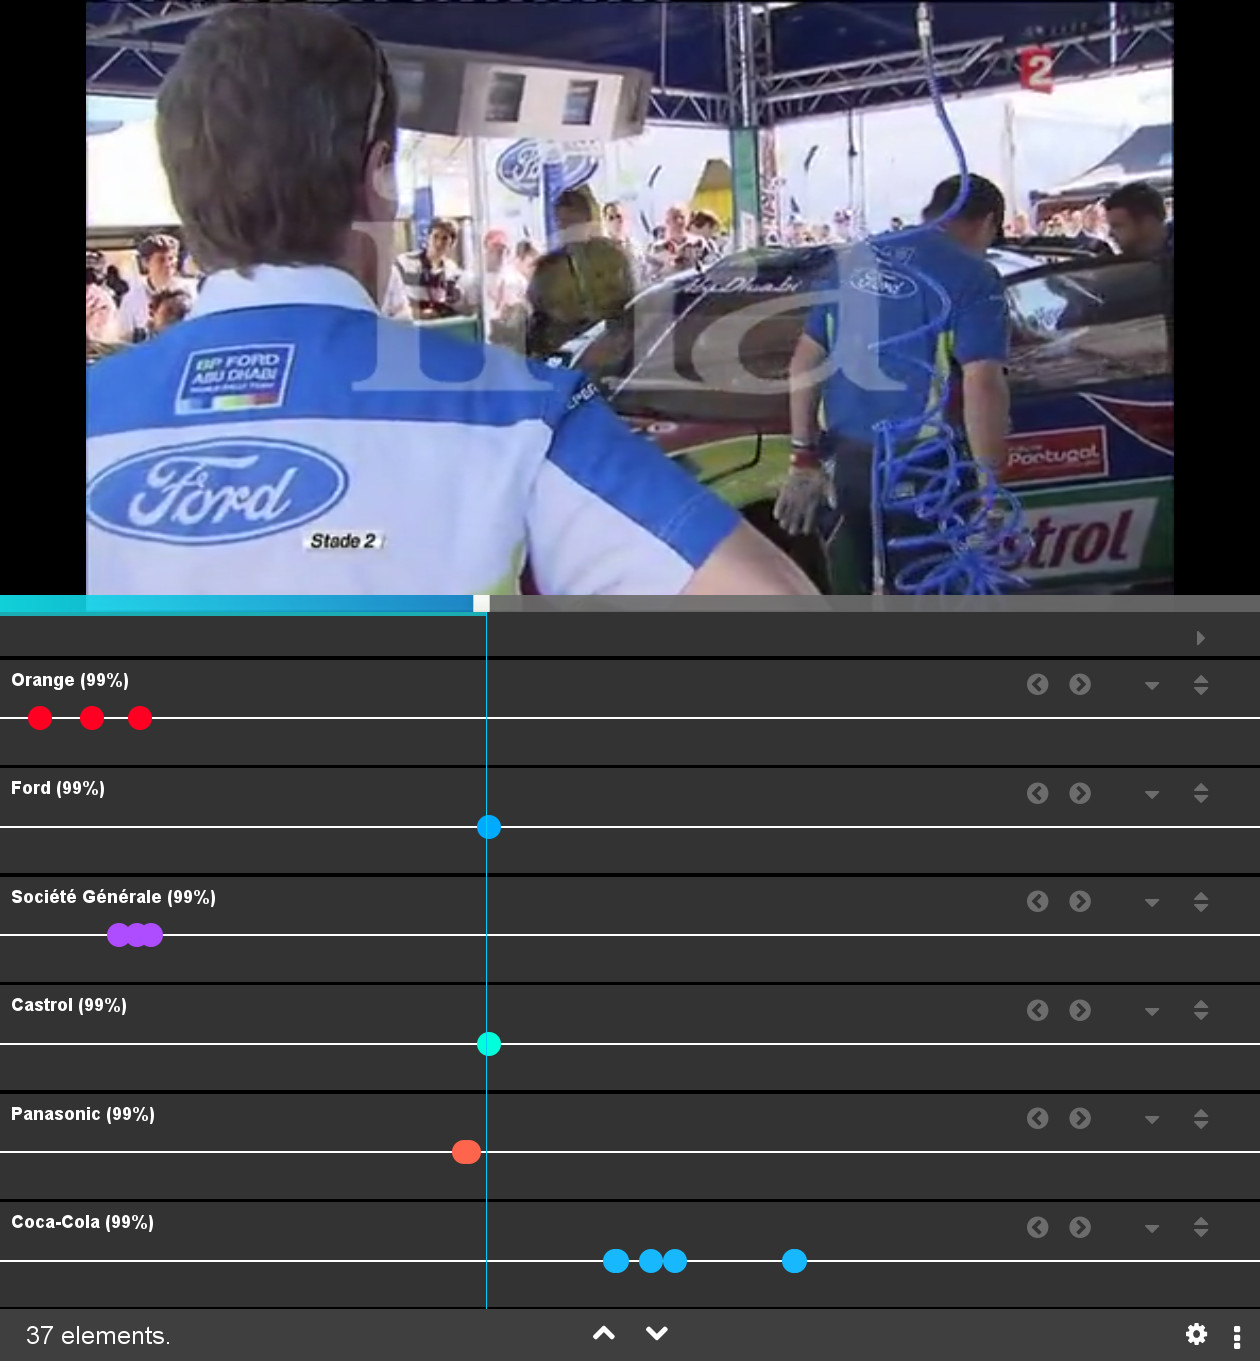
\includegraphics[width=10cm]{images/diginpix_resultat.jpg}
	\caption[Extraction des entités nommées d'un programme de France 2 avec DigInPix]{Extraction des entités nommées d'un programme de France 2 avec DigInPix [Source: \cite{institut_national_de_laudiovisuel_diginpix_nodate}]}
	\label{diginpix_result}
\end{figure}

Avec le projet du \index[ref]{led@Linked Enterprise Data (LED)!ldd@Lac de données (INA)}\index[ref]{modelisation@Modélisation!ldd@Lac de données (INA)}\ldd, la création de descriptions de contenus peut aller encore plus loin. En effet, le modèle de données unifié, comprenant l'ensemble des anciens référentiels de la \ac{ddcol}, permet de mettre en relation les données issues automatiquement d'un processus de traitement des vidéos par l'intelligence artificielle avec les concepts du \ldd. La segmentation automatique de vidéos\footnote{Le projet est SAAJ, Segmentation et Analyse Automatique des Journaux télévisés.} montre la diversité des utilisations possibles d'un référentiel quand celui-ci est uniforme et centralisé. Ce nouveau projet, au sein de celui du \ldd, débute en 2018 et conduit à la création de multiples outils, permettant tous une description automatique du contenu d'une vidéo --- les journaux télévisés et les chaînes d'information. Ainsi, la segmentation automatique par l'intelligence artificielle permet:
\begin{itemize}
	\item l'établissement d'une grille de programmation à partir des métadonnées fournies par les diffuseurs, les producteurs, \dots afin de déterminer les horaires prévus et habituels de chaque programme pour les chaînes d'information
	\item la classification automatique du programme ou des segments de programme selon une typologie précise --- plateau, présentateur, reportage, \dots
	\item la transcription des voix et de la parole, produisant ainsi un texte non formaté à partir duquel une description du contenu est effectuée avec des entités nommées qui en sont extraites et un alignement avec les entités de Wikidata
	\item l'océrisation des textes présents dans l'image, créant également un texte qui permet une description intellectuelle du contenu et un alignement des entités nommées avec Wikidata; cette océrisation concerne notamment les bandeaux des journaux télévisés dans lesquels le nom et la fonction de chaque personne sont indiqués
	\item la description automatique d'une image par un tagging d'entités nommées
	\item la reconnaissance de visages afin d'identifier le présentateur du journal télévisé, ou les protagonistes des vidéos
	\item la reconnaissance d'images et de logos, afin d'enrichir la description déjà précise de la vidéo ou du segment
\end{itemize} 

Chacun de ces outils fonctionne avec, ou en relation avec, un ou plusieurs référentiels: ils peuvent être internes, c'est à dire propres à l'\ac{ina}, ou bien externes comme Wikidata qui permet un enrichissement et une ouverture des métadonnées vers l'extérieur. Ces données générées automatiquement sont créées sous le modèle du \index[ref]{led@Linked Enterprise Data (LED)!ldd@Lac de données (INA)}\index[ref]{modelisation@Modélisation!ldd@Lac de données (INA)}\ldd et sont, par conséquent, en relation avec ses concepts. 

\subsection{\label{III-B-3-b}Faciliter et améliorer le catalogage des documents de l’\ac{ina} par l’extraction automatique de données}
\titreEntete{Faciliter et améliorer le catalogage des documents}

L'apport du projet SAAJ est une description fine et précise de l'ensemble d'une vidéo. Au-delà de la génération automatique de métadonnées dans le \index[ref]{led@Linked Enterprise Data (LED)!ldd@Lac de données (INA)}\index[ref]{modelisation@Modélisation!ldd@Lac de données (INA)}\ldd, il devient une aide pour le technicien de gestion des contenus multimédia de l'\ac{ina}. En effet, il n'a plus à créer les métadonnées associées au document, mais à superviser leur qualité et leur véracité: \og Le documentaliste « humain » est-il destiné à
passer du statut de producteur de données à celui de contrôleur de la qualité des fruits de l’automatisation ?\fg{}\footcite[p.134]{alquier_production_2017}. Cet aspect de contrôle qualité est un usage indirect des données générées automatiquement: il est positif pour la création précise, fine et complète de métadonnées sur un programme; mais il contraint à un changement de pratiques de catalogage, où l'humain n'a plus le rôle principal, qui est intellectuel, dans lequel il décrit le document et son contenu. \\

Cette amélioration et cette facilitation du travail de catalogage a lieu depuis des données nouvelles, générées par l'intelligence artificielle. Cependant, le contrôle de la qualité des métadonnées, et leur enrichissement, peuvent également passer par un traitement \textit{a posteriori}. En effet, l'apparition du Web sémantique et son adoption par un grand nombre d'institutions a poussé l'\ac{ina}, associé à d'autres institutions, à mener le projet Qualinca entre 2012 et 2015 afin \og d'améliorer la richesse, la cohérence et l’interopérabilité des métadonnées du système documentaire de l’Ina à travers la mise en œuvre d’une activité de recherche dans le domaine des techniques de liage de données\fg{}\footcite[p.129]{alquier_production_2017}. Qualinca repose sur de nombreux enjeux, comme la possibilité de partager des identifiants communs entre les différents métiers, l'amélioration des descriptions de contenus grâce aux données extérieures du \index[ref]{lod@Linked Open Data (LOD)}\ac{lod}, mais également d'effacer les ambiguïtés des termes des lexiques de l'\ac{ina}.\\

Se basant sur deux algorithmes, ProbFr et Agreg, Qualinca s'est surtout tourné vers les alignements de corpus de musique, et d'homonymes de personnes physiques et d'émissions. Dans cet alignement des homonymes avec le \index[ref]{lod@Linked Open Data (LOD)}\ac{lod}, la base \index[ref]{lod@Linked Open Data (LOD)!dbpedia@DBpédia}DBpedia --- Wikidata n'est né qu'en 2014 ---, les résultats sont peu exploitables et se heurtent, comme nous avons pu le constater lors de l'alignement des personnes physiques avec Wikidata, au langage naturel des fonctions que les algorithmes sont incapables de dépasser: sur 5000 \nP{Jacques}{Martin}, 667 différents ont été identifiés par les algorithmes\footcite[p.133]{alquier_production_2017}.\\

L'extraction automatique d'entités nommées a permis la création de nouvelles métadonnées, associées non pas au matériel ou aux données de diffusion mais au contenu intellectuel des vidéos, ainsi que l'apport d'une aide au \index[ref]{led@Linked Enterprise Data (LED)!ldd@Lac de données (INA)}\index[ref]{modelisation@Modélisation!ldd@Lac de données (INA)}catalogage par la qualité des entités fournies et leur précision.

\subsection{\label{III-B-3-c}Améliorer la valorisation des documents et offrir une meilleure expérience utilisateur}
\titreEntete{Améliorer la valorisation des documents}

La centralisation des données de l'\ac{ina} au sein du \index[ref]{led@Linked Enterprise Data (LED)!ldd@Lac de données (INA)}\index[ref]{modelisation@Modélisation!ldd@Lac de données (INA)}\ldd ouvre des possibilités pour la valorisation des documents auprès de tous les publics\footnote{Pour l'ensemble de l'offre disponible, voir la \reference{I-B}.}. D'abord, cette centralisation permet la création de multiples applications pour l'utilisateur, sans que cela ne modifie la structure des données\footnote{Voir \reference{annexe_lac} (\reference{lac_infra}).}; ainsi, la présence de l'\ac{ina} en est modifiée par l'apparition d'un \textit{hub} regroupant l'ensemble de l'offre numérique de l'Institut\footnote{\og L’autre grand défi posé à l’Institut, c’est celui de l’accessibilité de ses propositions. Les rassembler au sein d’un grand portail numérique, un hub qui offrira en quelques clics un accès renouvelé, simplifié et cohérent à l’ensemble des activités, contenus et services de l’Ina, est ainsi l’objectif qui mobilise aujourd’hui toute l’entreprise à l’horizon de 2019.\fg{} in \cite{vallet_ina_nodate}}.\\

Cette centralisation de l'offre est aussi présente pour les usages internes avec la création d'une nouvelle interface de consultation des métadonnées et des documents en eux-mêmes, Notilus, afin d'éviter la consultation croisée de multiples interfaces selon la provenance du document comme cela était le cas avant le \index[ref]{led@Linked Enterprise Data (LED)!ldd@Lac de données (INA)}\index[ref]{modelisation@Modélisation!ldd@Lac de données (INA)}\ldd. Par cette interface, le \ac{dl}, le \ac{da}, puis la \ac{dj} et l'ensemble des professionnels de l'\ac{ina}, ont accès aux mêmes données et aux mêmes documents, en un point unique, une interface de consultation qui reconstitue les instances du \ldd.\\

L'amélioration de l'expérience utilisateur est également une priorité dans une période où la modification des pratiques est radicale: ces pratiques sont quasiment toutes numériques et contraignent l'\ac{ina} à s'adapter. Si le site \url{https://www.ina.fr} est né dès 2009, le \index[ref]{led@Linked Enterprise Data (LED)!ldd@Lac de données (INA)}\index[ref]{modelisation@Modélisation!ldd@Lac de données (INA)}\ldd va pouvoir lui apporter d'importantes améliorations. En effet, la présence des référentiels y est limitée et restreint les possibilités de rebonds de la part de l'utilisateur\footnote{Voir \reference{inafr_result}.}. Ainsi, les liens des personnes au générique ne renvoient pas à une vedette personne de l'\ac{ina}, mais à des résultats de recherche sur le nom de cette personne. 
\begin{figure}[!h]
	\centering
	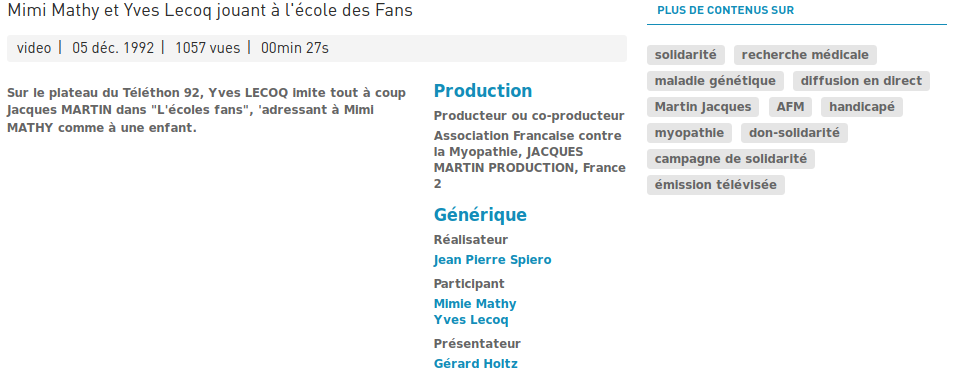
\includegraphics[width=13cm]{images/inafr_ecole_fans.png}
	\caption[Métadonnées associées à un document sur ina.fr]{Métadonnées associées à un document sur ina.fr [Source: \url{https://www.ina.fr/video/I11297765/mimi-mathy-et-yves-lecoq-jouant-a-l-ecole-des-fans-video.html}]}
	\label{inafr_result}
\end{figure}\\
Les possibilités offertes par le \ldd sont multiples et nous pouvons en imaginer certaines, basées sur le seul usage des concepts et de leurs relations, qui faciliteraient la recherche de l'utilisateur. Ainsi, comme pour la BnF, la création de vedettes de personnes est envisageable afin de regrouper en une même page les informations biographiques, ainsi que les documents liés (les instances) ou bien les thématiques principales (les concepts liés). Les termes d'indexation et de description des vidéos peuvent également être concernés par ce regroupement d'informations et de liens. Cependant, plus encore que ces regroupements de métadonnées, d'instances et de concepts relatifs à un concept, il est désormais possible, par les liens établis avec le \index[ref]{lod@Linked Open Data (LOD)}\ac{lod}, d'obtenir des informations manquantes et d'enrichir les données proposées à l'utilisateur: un lien peut être inséré, comme c'est le cas dans \index[ref]{lod@Linked Open Data (LOD)!viaf@VIAF}\index[ref]{autorites@Autorités!viaf@VIAF}\ac{viaf}, ou bien les champs peuvent être directement remplis sur la page HTML.\\

Ces possibilités ne sont envisageables que par la déconstruction de l'information dans le \ldd, permettant alors une grande modularité des données dans les usages qui en sont faits. Ces usages ne sont pas tous nés et le \index[ref]{led@Linked Enterprise Data (LED)!ldd@Lac de données (INA)}\index[ref]{modelisation@Modélisation!ldd@Lac de données (INA)}\ldd doit pouvoir permettre à l'\ac{ina} de les remplir sans avoir recours à un modification du modèle de données ou à la création d'une nouvelle de données. Ainsi, s'il est nécessaire de publier les données\footnote{Cet aspect semble difficile pour l'\ac{ina} en raison des données personnelles qui y sont conservées. Cependant, la loi de 2016 pour une République numérique (\cite{noauthor_loi_2016}) encourage à la publication des données de référence qui peuvent être réutilisées par d'autres services ou d'autres institutions.} sur le Web et plus particulièrement sur le Web de données, une représentation \index[ref]{echanges@Échanges!formats@Formats!rdf@RDF}\ac{rdf} est possible; avec la forte présence de l'\ac{ina} sur les réseaux sociaux, il peut être envisager de créer des publications automatiquement à partir de tags issus de concepts; \dots

%conclu
\bigskip
\bigskip
Le référentiel a atteint une place centrale dans le \ldd: l'ensemble des applications et des sites de l'Institut fonctionnent, ou vont fonctionner, depuis ce silo de métadonnées qui a été pensé selon la donnée et non plus selon les besoins. Ces derniers, évolutifs et dépendants de la période, ne peuvent pas tous être prédits, ce qui a conduit à la constitution d'un modèle de données souple et d'un processus intermédiaire de traitement de ces données, de manière à offrir à chaque application les données qui lui sont nécessaires.